\documentclass[a4paper,justified,final,twoside,nobib]{tufte-book}

\hypersetup{colorlinks}% uncomment this line if you prefer colored hyperlinks (e.g., for onscreen viewing)

\usepackage{mathtools} %added mathtools for piecewise functions

\usepackage{nameref} %added to reference sections by name

%%
% Book metadata
\title{A\\Machine Learning\\Handbook\thanks{Thanks to Edward R.~Tufte for his inspiration.}}
\author[]{}
\publisher{Publisher of This Book}

%%
% Automated bibliography management
\usepackage{natbib}
\usepackage{amsmath}
\usepackage{amssymb}
\setcitestyle{authoryear}

%%
% If they're installed, use Bergamo and Chantilly from www.fontsite.com.
% They're clones of Bembo and Gill Sans, respectively.
%\IfFileExists{bergamo.sty}{\usepackage[osf]{bergamo}}{}% Bembo
%\IfFileExists{chantill.sty}{\usepackage{chantill}}{}% Gill Sans

\usepackage{microtype}

%%
% For url line breaks
%\RequirePackage[hyphens]{url}\usepackage{hyperref}
\usepackage{url}
\def\UrlBreaks{\do\/\do-}

%%
% Describe algorithms using fancy pseudo code
\usepackage{algorithm}
\usepackage[noend]{algpseudocode}

%%
% Just some sample text
\usepackage{lipsum}
\usepackage{soul}
%%
% For nicely typeset tabular material
\usepackage{booktabs}
\usepackage{pdfpages}

%%
% For graphics / images
\usepackage{graphicx}
\setkeys{Gin}{width=\linewidth,totalheight=\textheight,keepaspectratio}
\graphicspath{{graphics/}}

% The fancyvrb package lets us customize the formatting of verbatim
% environments.  We use a slightly smaller font.
\usepackage{fancyvrb}
\fvset{fontsize=\normalsize}

%%
% Prints argument within hanging parentheses (i.e., parentheses that take
% up no horizontal space).  Useful in tabular environments.
\newcommand{\hangp}[1]{\makebox[0pt][r]{(}#1\makebox[0pt][l]{)}}

%%
% Prints an asterisk that takes up no horizontal space.
% Useful in tabular environments.
\newcommand{\hangstar}{\makebox[0pt][l]{*}}

%%
% Prints a trailing space in a smart way.
\usepackage{xspace}
% bold in maths equations
\usepackage{bm}

%%
% Some shortcuts for Tufte's book titles.  The lowercase commands will
% produce the initials of the book title in italics.  The all-caps commands
% will print out the full title of the book in italics.
\newcommand{\vdqi}{\textit{VDQI}\xspace}
\newcommand{\ei}{\textit{EI}\xspace}
\newcommand{\ve}{\textit{VE}\xspace}
\newcommand{\be}{\textit{BE}\xspace}
\newcommand{\VDQI}{\textit{The Visual Display of Quantitative Information}\xspace}
\newcommand{\EI}{\textit{Envisioning Information}\xspace}
\newcommand{\VE}{\textit{Visual Explanations}\xspace}
\newcommand{\BE}{\textit{Beautiful Evidence}\xspace}
\newcommand{\ics}{\smallcaps{ICS5110 Applied Machine Learning\xspace}}

\newcommand{\TL}{Tufte-\LaTeX\xspace}

% Prints the month name (e.g., January) and the year (e.g., 2008)
\newcommand{\monthyear}{%
  \ifcase\month\or January\or February\or March\or April\or May\or June\or
  July\or August\or September\or October\or November\or
  December\fi\space\number\year
}

% Prints an epigraph and speaker in sans serif, all-caps type.
\newcommand{\openepigraph}[2]{%
  %\sffamily\fontsize{14}{16}\selectfont
  \begin{fullwidth}
  \sffamily\large
  \begin{doublespace}
  \noindent\allcaps{#1}\\% epigraph
  \noindent\allcaps{#2}% author
  \end{doublespace}
  \end{fullwidth}
}

% Inserts a blank page
\newcommand{\blankpage}{\newpage\hbox{}\thispagestyle{empty}\newpage}

\usepackage{units}

% Typesets the font size, leading, and measure in the form of 10/12x26 pc.
\newcommand{\measure}[3]{#1/#2$\times$\unit[#3]{pc}}

% Macros for typesetting the documentation
\newcommand{\hlred}[1]{\textcolor{Maroon}{#1}}% prints in red
\newcommand{\hangleft}[1]{\makebox[0pt][r]{#1}}
\newcommand{\hairsp}{\hspace{1pt}}% hair space
\newcommand{\hquad}{\hskip0.5em\relax}% half quad space
\newcommand{\TODO}{\textcolor{red}{\bf TODO!}\xspace}
\newcommand{\ie}{\textit{i.\hairsp{}e.}\xspace}
\newcommand{\eg}{\textit{e.\hairsp{}g.}\xspace}
\newcommand{\na}{\quad--}% used in tables for N/A cells
\providecommand{\XeLaTeX}{X\lower.5ex\hbox{\kern-0.15em\reflectbox{E}}\kern-0.1em\LaTeX}
\newcommand{\tXeLaTeX}{\XeLaTeX\index{XeLaTeX@\protect\XeLaTeX}}
% \index{\texttt{\textbackslash xyz}@\hangleft{\texttt{\textbackslash}}\texttt{xyz}}
\newcommand{\tuftebs}{\symbol{'134}}% a backslash in tt type in OT1/T1
\newcommand{\doccmdnoindex}[2][]{\texttt{\tuftebs#2}}% command name -- adds backslash automatically (and doesn't add cmd to the index)
\newcommand{\doccmddef}[2][]{%
  \hlred{\texttt{\tuftebs#2}}\label{cmd:#2}%
  \ifthenelse{\isempty{#1}}%
    {% add the command to the index
      \index{#2 command@\protect\hangleft{\texttt{\tuftebs}}\texttt{#2}}% command name
    }%
    {% add the command and package to the index
      \index{#2 command@\protect\hangleft{\texttt{\tuftebs}}\texttt{#2} (\texttt{#1} package)}% command name
      \index{#1 package@\texttt{#1} package}\index{packages!#1@\texttt{#1}}% package name
    }%
}% command name -- adds backslash automatically
\newcommand{\doccmd}[2][]{%
  \texttt{\tuftebs#2}%
  \ifthenelse{\isempty{#1}}%
    {% add the command to the index
      \index{#2 command@\protect\hangleft{\texttt{\tuftebs}}\texttt{#2}}% command name
    }%
    {% add the command and package to the index
      \index{#2 command@\protect\hangleft{\texttt{\tuftebs}}\texttt{#2} (\texttt{#1} package)}% command name
      \index{#1 package@\texttt{#1} package}\index{packages!#1@\texttt{#1}}% package name
    }%
}% command name -- adds backslash automatically
\newcommand{\docopt}[1]{\ensuremath{\langle}\textrm{\textit{#1}}\ensuremath{\rangle}}% optional command argument
\newcommand{\docarg}[1]{\textrm{\textit{#1}}}% (required) command argument
\newenvironment{docspec}{\begin{quotation}\ttfamily\parskip0pt\parindent0pt\ignorespaces}{\end{quotation}}% command specification environment
\newcommand{\docenv}[1]{\texttt{#1}\index{#1 environment@\texttt{#1} environment}\index{environments!#1@\texttt{#1}}}% environment name
\newcommand{\docenvdef}[1]{\hlred{\texttt{#1}}\label{env:#1}\index{#1 environment@\texttt{#1} environment}\index{environments!#1@\texttt{#1}}}% environment name
\newcommand{\docpkg}[1]{\texttt{#1}\index{#1 package@\texttt{#1} package}\index{packages!#1@\texttt{#1}}}% package name
\newcommand{\doccls}[1]{\texttt{#1}}% document class name
\newcommand{\docclsopt}[1]{\texttt{#1}\index{#1 class option@\texttt{#1} class option}\index{class options!#1@\texttt{#1}}}% document class option name
\newcommand{\docclsoptdef}[1]{\hlred{\texttt{#1}}\label{clsopt:#1}\index{#1 class option@\texttt{#1} class option}\index{class options!#1@\texttt{#1}}}% document class option name defined
\newcommand{\docmsg}[2]{\bigskip\begin{fullwidth}\noindent\ttfamily#1\end{fullwidth}\medskip\par\noindent#2}
\newcommand{\docfilehook}[2]{\texttt{#1}\index{file hooks!#2}\index{#1@\texttt{#1}}}
\newcommand{\doccounter}[1]{\texttt{#1}\index{#1 counter@\texttt{#1} counter}}

% Generates the index
\usepackage{makeidx}
\makeindex

\usepackage{tikz}
\usepackage{makecell}

\begin{document}
%% Cover Page
\begingroup
\thispagestyle{empty}
\begin{tikzpicture}[remember picture,overlay]
\node[inner sep=0pt, outer sep=0pt] (background) at (current page.center) {\includegraphics[width=\paperwidth]{cover/cover_oreilly_style.pdf}};
\end{tikzpicture}
\vfill
\endgroup

% Front matter
\frontmatter

% r.3 full title page
%% \maketitle


% v.4 copyright page
\newpage
\begin{fullwidth}
~\vfill
\thispagestyle{empty}
\setlength{\parindent}{0pt}
\setlength{\parskip}{\baselineskip}
\begin{figure*}[h]
	\includegraphics[width=2.5in]{UMLOGO_redRGB.png}%
\end{figure*}

\par Copyright \copyright\ \the\year\ \ics\ class of 2018/9, University of Malta.










\par\smallcaps{Jean-Paul Ebejer, Dylan Seychell, Lara Marie Demajo, Daniel Farrugia, Keith Mintoff, Franco Cassar Manghi, David Farrugia, Ivan Salomone, Andrew Cachia, Jake J.\ Dalli, Joseph Azzopardi, Natalia Mallia, Mark Muscat, Stefan Cassar, Patrick Bezzina, Dylan Vassallo, Brian Pace, George Eduardo Buckup Sulzbeck, Katrin Jansen, Aliia Erofeeva, Michael Filletti, Neil Farrugia, Claire Galea, Albert Bezzina, Philip Mifsud, Neil Micallef, Matthew Farrugia, Samuel Mizzi, Aaron Grech, Peter Incorvaja} %TODO


\par Licensed under the Apache License, Version 2.0 (the ``License''); you may not
use this file except in compliance with the License. You may obtain a copy
of the License at \url{http://www.apache.org/licenses/LICENSE-2.0}. Unless
required by applicable law or agreed to in writing, software distributed
under the License is distributed on an \smallcaps{``AS IS'' BASIS, WITHOUT
WARRANTIES OR CONDITIONS OF ANY KIND}, either express or implied. See the
License for the specific language governing permissions and limitations
under the License.\index{license}

\par\textit{First printing, \monthyear}
\end{fullwidth}

% r.5 contents
\tableofcontents

%%\listoffigures

%%\listoftables

% r.9 introduction
\cleardoublepage
\chapter{Introduction}

This book explains popular Machine Learning terms.  We focus to explain each term comprehensively, through the use of examples and diagrams.  The description of each term is written by a student sitting in for \ics\footnote{\url{https://www.um.edu.mt/courses/studyunit/ICS5110}} at the University of Malta (class 2018/2019).  This study-unit is part of the MSc.\ in AI offered by the Department of Artificial Intelligence, Faculty of ICT.

%%
% Start the main matter (normal chapters)
\mainmatter

%% JP's example file -- file must be stored in directory "terms" and have
%% the term and initials of the student in the filename.
\input{terms/activationfunctions_km.tex}
\chapter{Bayesian Models in Machine Learning}\index{Bayesian Models|(}

Many machine learning\index{Machine Learning} techniques employ probability theory to make the best decisions given some data. Probabilistic approaches are often also summarised under the term ``Bayesian approaches"\index{Bayesian Models!Bayesian approaches} \citep{Murphy2012}. The following chapter will provide an overview of the underlying theorem as well as the most popular classifier based on said theorem.

\section{Bayes' Theorem} \label{sec:bayes_theorem}

Bayes' Theorem\index{Bayesian Models!Bayes' Theorem} describes how to calculate the so-called posterior probability of an event $A$ given our observed evidence $B$, that is $P(A|B)$. It is derived from the definition of conditional probabilities \eqref{eq:cond_prob}. The probability of an event $B$ to occur given that the event $A$ already has occurred is defined as the probability of the intersection of the two events $A$ and $B$ divided by the probability of the event $A$ \citep{Murphy2012}:

\begin{gather}
    P(B|A) = \frac{P(A \cap B)}{P(A)} \label{eq:cond_prob}
\end{gather}
The probability of the intersection of the two events $A$ and $B$ can be rewritten as \eqref{eq:prob_intersect_a}. However, since $P(A \cap B)$ is equal to $P(B \cap A)$, it can be rewritten as \eqref{eq:prob_intersect_b}, as well \citep{Manning2009}. 

\begin{gather}
    P(A \cap B) = P(A) P(B|A) \label{eq:prob_intersect_a}
\end{gather}
\begin{gather}
    P(B \cap A) = P(B) P(A|B) \label{eq:prob_intersect_b}
\end{gather}
Consequently, Bayes' Theorem can be derived as follows:


\begin{align}
    P(B|A)  &= \frac{P(A \cap B)}{P(A)}
           = \frac{P(B \cap A)}{P(A)}
            = \frac{P(B) P(A|B)}{P(A)} \notag\\
    \Leftrightarrow P(A|B) &= \frac{P(B|A) P(A)}{P(B)} \label{eq:BT_derived}
\end{align}
$P(A|B)$ is the aforementioned posterior probability, $P(B|A)$ the likelihood of event $B$ given event $A$, $P(A)$ the prior probability of event $A$, and $P(B)$ the so-called marginal, that is the likelihood of an independent occurrence of event $B$ \citep{Manning2009, Rijsbergen1979}.

\section{Na\"ive Bayes Classification Algorithm} \label{sec:NB_class}

Intuitively, Bayes' Theorem can be used to calculate the probability of an hypothesis being true given some observed evidence \citep{Manning2009, martin2018speech, Rijsbergen1979} - it is a structured way of integrating all available information into an estimation of the truth of that hypothesis. However, it can also be used as a classification method \citep{Manning2009, martin2018speech, Murphy2012, Rijsbergen1979}: The instance to be classified (such as an email, a web page, or a newspaper article) is taken to be the ``observed evidence" for that instance to belong to a certain class. For example, the content of an email is taken to be the information available to classify that email as spam or ham. Bayes' Theorem is applied to the conditional probability $P(c|d)$ of a given document $d$ belonging to a certain class $c$, resulting in \eqref{eq:NB_class_der}. The denominator $P(d)$ can be dropped, since the prior probability of a document to occur is the same for all possible classes and does not have any effect on the final classification decision \citep{martin2018speech}. Ultimately, the result is \eqref{eq:NB_class}.

\begin{gather}
    P(c|d) = \frac{P(d|c)P(c)}{P(d)} \label{eq:NB_class_der}
\end{gather}

\begin{gather}
    P(c|d) \propto P(c) \prod_{1 \leq k \leq n_{d}} P(t_{k}|c)\label{eq:NB_class}
\end{gather}
\eqref{eq:NB_class} can be read as the probability of a given document $d$ belonging to a certain class $c$ being proportional to the prior probability of a document occurring in class $c$ multiplied by the probability of that class $c$ having generated a document consisting of all the terms $t_{k}$ in $d$. Na\"ive Bayes classifiers\index{Bayesian Models!Na\"ive Bayes classifier} are also called generative classifiers \citep{Murphy2012}: Given a specific observation $d$, they return the class $c$ that is most likely to have generated said observation - also called the maximum a posteriori (MAP) class.

The two parameters needed to calculate $P(c|d)$, $P(c)$ and $P(t_{k}|c)$, are obtained via approximations from the training set, based on maximum likelihood estimations (MLE)\index{Maximum likelihood estimation} \citep{Manning2009, martin2018speech}. For the prior probability $P(c)$, the estimate is as follows:
\begin{gather}
    \hat{P}(c) = \frac{N_{c}}{N}\label{eq:prior_est},
\end{gather}
which is the number of documents in the training set belonging to class $c$ divided by the total amount of documents in the training set \citep{Manning2009, martin2018speech}. Similarly, the probability of a term $t_{k}$ occurring in a document of class $c$ is obtained like this:
\begin{gather}
    \hat{P}(t_{k}|c) = \frac{T_{ct}}{\sum_{t' \in V} T_{ct'}}\label{eq:likelihood_est},
\end{gather}
which is the number of times a term $T$ appears in documents of class $c$ divided by the number of times that term appears in the vocabulary $V$, i.e. in all documents of the training set \citep{martin2018speech, Manning2009}.

These approximations pose two problems. First of all, the multiplication of all the conditional probabilities $P(t_{k}|c)$ may result in a so-called floating-point underflow \citep{Manning2009}. In order to avoid this, Na\"ive Bayes classifiers\index{Bayesian Models!Na\"ive Bayes classifier} usually do not calculate the product over $P(t_{k}|c)$, but the sum over the log values of $P(t_{k}|c)$ (see \eqref{eq:log_NB_class}). Using the log values instead of the original ones does not interfere with the final classification decision in any way: The class with the highest log probability is still the one most likely to have generated the given document.

\begin{gather}
    P(c|d) \propto P(c) \prod_{1 \leq k \leq n_{d}} \log P(t_{k}|c)\label{eq:log_NB_class}
\end{gather}

The second problem encountered by the estimations above is data sparseness, resulting in terms not occurring in documents of particular classes in the training set. The preferred solution is to eliminate the resulting zeros by using add-one or Laplace-smoothing (see \eqref{eq:laplace}, with $B' = |V|$, the length of the vocabulary), assuming that each and every relevant term occurs at least once in a corpus \citep{Manning2009}. % Words that are unknown altogether (i.e. that do not appear in the training set at all) are typically removed from consideration \citep{}.

\begin{gather}
    \hat{P}(t_{k}|c)    = \frac{T_{ct} + 1}{\sum_{t' \in V} (T_{ct'} + 1)}
                        = \frac{T_{ct} + 1}{(\sum_{t' \in V} T_{ct'}) + B'} \label{eq:laplace}
\end{gather}

\section{Na\"ive Assumptions} \label{sec:naive}

While the calculations above appear to be straightforward, they pose a problem in terms of their feasibility, especially regarding big sets of data. Relating individual probabilities to all terms of a document – even to those occurring multiple times in different positions – increases the number of parameters dramatically and requires huge sets of training data, which are almost never available. Naïve Bayes\index{Bayesian Models!Na\"ive Bayes classifier} offers solutions to this problem via two rather na\"ive assumptions giving the classifier its name \citep{Manning2009, martin2018speech}. 

Hence, Na\"ive Bayes classifiers\index{Bayesian Models!Na\"ive Bayes classifier} assume the bag of words model\index{Bag of words model} for all terms in a document, that is they assume the probability of a term to be the same, regardless of its position in the document. This is also called the positional independence assumption \citep{Manning2009, martin2018speech}.

The second assumption is called the conditional independence assumption. It simplifies the calculation further by proposing that all terms in a document are independent of one another, i.e. the occurrence of a specific term does not make it any more likely for another, possibly related term to appear in the same document. Obviously, the exact opposite is true - in reality, the terms in a document are indeed dependent on one another. However, Na\"ive Bayes classifiers\index{Bayesian Models!Na\"ive Bayes classifier} still offer accurate classification decisions, regardless of the inaccuracies in their probability estimations \citep{Manning2009, martin2018speech}.  

\section{Conclusion}

The classification method\index{classification} described just now is just one of the versions of Bayesian classifiers\index{Bayesian Models!Na\"ive Bayes classifier}, called the multinomial Na\"ive Bayes classifier\index{Bayesian Models!Na\"ive Bayes classifier}. One alternative is the Bernoulli model \citep{Manning2009}. In order to arrive at a classification decision, the Bernoulli model uses only binary information regarding the occurrence ($1$) or absence ($0$) of a term in a document. This often leads to errors regarding the classification of long documents, since the actual number of occurrences of a term are not taken into account, which is why the multinomial model is preferred.

\index{Bayesian Models|)}
\input{terms/classification_cg.tex}
\input{terms/conceptdrift_mf.tex}
\input{terms/confusionmatrix_df.tex}
\input{terms/convolution_gebs.tex}
\input{terms/crossvalidation_lmd.tex}
\chapter{Dimensionality Reduction}
\label{ch:dimensionality reduction}\index{dimensionality reduction|(}

As the volume of data collected increased, several machine learning approaches have been formulated to identify patterns and perform predictions from this data. Apart from their large volume, these datasets constitute of a large number of variables. This high dimensionality within the data presented challenges such as excessive computational costs and increased memory requirements \citep{featureselectionforhighdimensionaldata}. 

For these reasons, prior to applying any of these data mining techniques, pre-processing mechanisms are normally applied on the data. These methods include dimensionality reduction which is the process in which the large number of input variables are reduced to a smaller set of features \citep{Sorzano2014}.

\citet{DataShrinkingBasedFeatureRankingforProteinClassification} mention \textit{feature selection}\index{dimensionality reduction!feature selection} and \textit{feature extraction}\index{dimensionality reduction!feature extraction} as two possible methods which reduce the dimensionality of the data. Feature selection involves selecting only the relevant features of the dataset, whilst ignoring the remaining features \citep{DataShrinkingBasedFeatureRankingforProteinClassification}. 

On the other hand, feature extraction techniques are applied to construct a feature vector with lower dimensionality. Linear Discriminant Analysis (LDA) and Principal Component Analysis (PCA) are two common techniques applied for feature extraction, in which a linear transformation matrix is used to project the original features to a new feature space \citep{Wang2003}. 

\section{Random Forests}\index{dimensionality reduction!random forests}

\citet{Breiman2001} introduced Random Forests (RF) as an algorithm for \textit{classification}\index{dimensionality reduction!random forests!classification} and \textit{regression}\index{dimensionality reduction!random forests!regression} problems. However, this method is also useful in determining feature importance or irrelevance, thus widely used for variable selection \citep{Genuer2010}.

The concept behind RFs involves the iterative construction of a number of binary \textit{decision trees}\index{dimensionality reduction!random forests!decision trees}, which have a low degree of correlation \citep{Genuer2010}. In each iteration, a random sample is extracted from the training sample on which the decision tree will be trained. During training, each split involves randomly selecting $k$ features from the original feature vector $P$, where $k < P$. Data is split using the best feature out of the selected $k$ features. Once the separate decision trees, also referred to as random forests, are constructed, each tree can be used to predict outcomes for new samples. In classification problems, these outcomes are then averaged to obtain the final prediction \citep{kuhn2013applied}. 

\citet{Diaz-Uriarte2006} perform feature selection using a RF approach to select a smaller set of features that can still provide effective predictions in classification or regression problems. In their strategy, variable importances are initially calculated within each iteration. The variables with the smallest importances are eliminated and a new forest is then constructed using the remaining high importance variables. Finally, the prediction error of each forest, also referred to as the out-of-bag (OOB) error rate, is calculated. The features belonging to forests with the smallest error in prediction, are selected as the final variables \citep{Diaz-Uriarte2006}.

\citet{Strobl2007} discuss that RFs are not ideal for feature selection when the features to be used for prediction constitute of a mixture of categorical and continuous values. Moreover, the variable importances measures are unreliable in cases when the number of categories for categorical predictors vary in the sample set.

\section{Genetic Algorithms}\index{dimensionality reduction!genetic algorithms}

Genetic algorithms (GA) are a commonly used technique in feature selection, which aims at minimizing the feature space by eliminating unimportant variables and keeping those which maximize accuracy in predictions. Introduced by \citet{Holland1962}, GA works using a procedure which mimics the theory of evolution, in which a population is manipulated to generate offsprings which form the new generation. 

In GA's, a population is made up of a set of individuals (samples from a sample space), which are represented using binary strings, and referred to as \textit{chromosomes}\index{dimensionality reduction!genetic algorithms!chromosomes}. Each chromosome is composed of a set of features, which are called \textit{genes}\index{dimensionality reduction!genetic algorithms!genes} \citep{Siedlecki1989}. A \textit{fitness function}\index{dimensionality reduction!genetic algorithms!fitness function} is applied to each individual to determine the fittest individuals within the population. GA then applies selection to obtain the fittest individuals. Pairs of individuals, referred to as parents, are then constructed from the selected individuals, and crossover is performed. Crossover involves generating offsprings from the identified parents by exchanging information amongst the parent pairs. Mutation, which is applied to increase the diversity within the population, entails that one or more bits are randomly flipped to generate a different offspring. GA repeatedly perform this process, also referred to as a generation, until a stopping condition is met \citep{Chaikla}. 

In feature selection, the individual considered as the fittest from the new population obtained is used to determine the features with the highest importance. Genes with value '1' in the obtained chromosome are considered as the features to be used for predictions \citep{sivanandam2007introduction}.


\section{Principal Component Analysis}\index{dimensionality reduction!principal component analysis}

\citet{jolliffe2002principal} introduces PCA as the technique which aims ''to reduce the dimensionality of a data set consisting of a large number of interrelated variables, while retaining as much as possible of the variation present in the data set.'' PCA aims to transform a set of correlated variables $P$ into a set of uncorrelated $k$ variables, where $k < P$ and the $k$ variables maintain the majority of the information in $P$. 

Prior to applying PCA, the dataset is adjusted such that the means of the original variables are subtracted from the observations, to produce a dataset with mean zero \citep{jackson2005user}. PCA works by initially constructing the \textit{covariance matrix}\index{dimensionality reduction!principal component analysis!covariance matrix} of the data \citep{Guan2009}. A high covariance value indicates that the variables are correlated, whereas a zero value indicates that no correlation exists between the variables. Moreover, the covariance between $x$ and $y$ is equal to the variance of $x$, when $x = y$. 

\begin{marginfigure}
	\begin{equation*}
        \begin{pmatrix} cov(x, x) & cov(x, y) & cov(x, z) \\ cov(y, x) & cov(y, y) & cov(y, z) \\ cov(z, x) & cov(z, y) & cov(z, z)
        \end{pmatrix}
\end{equation*}
\caption{Covariance Matrix.}
\label{fig:covarianceMatrix}
\end{marginfigure}

The variance between features is indicated by the diagonal values of a covariance matrix (Figure~\ref{fig:covarianceMatrix}), whilst the off-diagonal values refer to the covariance between the features. High values in the off-diagonal terms indicate that high redundancy exists, and thus the covariance matrix must be diagonalized to minimize the correlations between the features. 

The resultant diagonalized covariance matrix is used to calculate the \textit{eigenvalues}\index{dimensionality reduction!principal component analysis!eigenvalues} and \textit{eigenvectors}\index{dimensionality reduction!principal component analysis!eigenvectors}. The eigenvectors refer to the direction in which the data varies, and these are ordered such that the ones with the highest eigenvalues are chosen as the principal components of the data. Eventually, the selected vectors are kept to form a \textit{feature vector}\index{dimensionality reduction!principal component analysis!feature vector}, which will be used to construct the new dataset with lower dimensionality, as in Equation~\ref{newDataSet} 


\begin{equation}\label{newDataSet}
	New Dataset = FeatureVector^T x AdjustedData^T 
	\end{equation}

Equation~\ref{newDataSet} multiplies the transpose of the feature vector by the transpose of the mean adjusted data, to obtain the original data with smaller dimensionality \citep{jackson2005user}.

\section{Multi-dimensional scaling}\index{dimensionality reduction!multi-dimensional scaling}

Multi-dimensional scaling (MDS) is another dimensionality reduction technique which similar to PCA seeks to obtain a data set with lower dimensions. MDS aims at finding a configuration in which the distances between points on a dimensional space are as close as possible to the dissimilarities between the points. Different techniques of MDS exist which differ in the way that points are matched to dissimilarities. In \textit{Metric MDS}\index{dimensionality reduction!multi-dimensional scaling!metric MDS}, ''dissimilarities between objects will be in numerical and distance''. Classical scaling is one such technique which aims at finding a configuration in which the dissimilarities are equal to Euclidean distances. Another technique is least squares scaling in which the dissimilarities are transformed into distances using a function, and the configuration space is obtained by minimising this function. On the other hand, \textit{Non-Metric MDS}\index{dimensionality reduction!multi-dimensional scaling!non-metric MDS} seeks a transformation which preserves the rank order of the dissimilarities \citep{cox2000multidimensional}.

\section{Linear Discriminant Analysis }\index{dimensionality reduction!linear discriminant analysis}

LDA is a supervised dimensionality reduction technique which produces a lower dimensionality feature space in which a feature vector belonging to a class is distinguishable from that of the other classes \citep{Sharma2015}. Figure~\ref{fig:dimensionalityReduction} depicts the projection of a two-dimensional feature vector to a one-dimensional feature space. $C_1$, $C_2$ and $C_3$ denote the three different classes being used within the feature vectors. By projecting the feature vectors onto line \^{W}, which represents one dimension, it is noted that a strong relationship exists between the feature vectors of the three classes. LDA seeks an orientation which strongly separates the feature vectors of one class from those belonging to other classes. This orientation can be obtained by rotating \^{W}, resulting in projection $W$, where the feature vectors of the classes are highly separated. Algorithmically, Fisher's criterion is maximized to obtain the required one-dimensional feature vector $W$.

\begin{marginfigure}
	\includegraphics{graphics/dimensionality_reduction/DimensionalityReductionLDA.png}
	\caption{
		Projection of a two-dimensional feature vector to a one-dimensional feature space. Adapted from \citet{Sharma2015}.
	}
	\label{fig:dimensionalityReduction}
  \end{marginfigure}

Feature extraction using LDA \citep{Sharma2015,Huang2002} works by initially calculating the separability between the mean values of each class.

\begin{equation}
	\label{betweenClassMatrix}
	S_B = \sum^{c}_{i=1}n_{i}(\mu_i - \mu)(\mu_i - \mu)^T
	\end{equation}

This is referred to as the \textit{between-class matrix}\index{dimensionality reduction!linear discriminant analysis!between-class matrix} and is represented by Equation~\ref{betweenClassMatrix}, where $c$ is the number of classes, $n_i$ is the number of samples for the $i^{th}$ class, $\mu_i$ is the mean for the $i^{th}$ class and $\mu$ is the total mean of all samples.

\begin{equation}
	\label{distanceBetweenMeanAndSampleMatrix}
	S_W = \sum^{c}_{j=1}\sum^{n_j}_{i=1}(x_{ij} - \mu_j)(x_{ij} - \mu_j)^T
	\end{equation}

Following this, the \textit{within-class matrix}\index{dimensionality reduction!linear discriminant analysis!within-class matrix} is calculated using Equation~\ref{distanceBetweenMeanAndSampleMatrix}, where $c$ is the number of classes, $n_j$ is the number of samples for the $j^{th}$ class, $x_{ij}$ is the $i^{th}$ sample in the $j^{th}$ class, and $\mu_j$ is the mean for the $j^{th}$ class. This matrix indicates the distance between the mean and sample values for each class. Finally, a \textit{transformation matrix}\index{dimensionality reduction!linear discriminant analysis!transformation matrix} $W$ which maximizes the between-class variance and minimizes the within-class variance should be constructed.

\begin{marginfigure}
	\begin{equation}
		\label{FishersCriterion}
		\arg\max_{w} \frac{W^T S_B W}{W^T S_W W}
		\end{equation}
	
	\begin{equation}
		\label{FishersCriterion2}
		S_W W = \lambda S_B W
		\end{equation}	
\end{marginfigure}


Fisher's criterion, shown in Equation~\ref{FishersCriterion} is used to obtain the maximum ratio of the between-class matrix (denoted by $S_B$) and within class matrix (represented by $S_W$). 
By transforming the latter into Equation~\ref{FishersCriterion2}, where $\lambda$ denotes the eigenvalues, eigenvectors and the corresponding eigenvalues of $W$ may be calculated. A lower dimensional space is constructed by selecting the eigenvectors having the highest eigenvalues. 

\index{dimensionality reduction|)}
\input{terms/empiricalriskminimisation_nf.tex}
\input{terms/ensemblemethods_dv.tex}
\input{terms/evaluationmethods_ae.tex}
\input{terms/featureselection_ab.tex}
\input{terms/generativemodels_pm.tex}
\input{terms/hyperparameters_nm.tex}
\chapter{Long Short-Term Memory}
\label{ch:lstm}

\index{lstm|(}

Some problems in Machine Learning, especially NLP-focused tasks, generally require some sort of \textbf{context} from previous iterations to form a more comprehensive understanding of the problem it is being given. 

When facing context-heavy sentences such, as, ``I am from Malta, and I speak \textit{Maltese}'', most models became unable to forge enough contextual clues\index{Contextual clues} in order to determine the nationality despite such clues, or \textbf{long-term dependencies}, being given earlier in the sentence \citep{bengio94}.

In order to solve this problem, \citet{hochreiter1997long} proposed the Long Short-Term Memory network, or LSTM. 

\section{LSTM Architecture}
This module is a type of Recurrent Neural Network (RNN), that is, a repeated chained module, with a gradient-based unit applied. The main difference is that the repeated module itself is different, with the LSTM module being composed of a series of gates named the \textbf{input gate}, \textbf{hidden gate}, \textbf{forget gate}, and \textbf{output gate}, as described in Figure~\ref{fig:lstm_architecture}.

\begin{figure*}
	\centering
	\includegraphics[width=0.6\linewidth]{graphics/lstm/lstm.png}
	\caption{
		Architecture of standard LSTM module. Adapted from: \citet{olah_2015}
	}
	\label{fig:lstm_architecture}
\end{figure*}

The traversal from one gate to another is handled through a number of \textbf{activation functions}, which have been discussed in a previous chapter. The LSTM framework uses three main functions:

{$\sigma _{g}$} - denoting the Sigmoid Function\index{Sigmoid Function} \citep{DavidE.Rumelhart1986Lrbb}.
{$\sigma _{c}$} - denoting the Hyperbolic Tangent Function.\index{Hyperbolic Tangent Function}
{$\sigma _{h}$} - also denotes the Hyperbolic Tangent Function in the case of the hidden gate, and implies that {$\sigma _{h}(x)=x$}.

In order for the LSTM module to learn, backpropagation\index{LSTM Backpropagation} is implemented in the form of the Constant Error Carousel (CEC)\index{Constant Error Carousel} function, which updates the hidden gate {$h_{t}$} through the following equations:

\begin{itemize}
	\setlength{\itemsep}{1pt}
	\setlength{\parskip}{0pt}
	\setlength{\parsep}{0pt}
	\item {$h_{t}$} -  the hidden state, denoted by 
	\begin{equation} \label{LSTM CEC}
	h_{t} = o_{t} \circ tanh(c_{t})
	\end{equation}
	where {$\circ$} implies the Hadamard Product (element-wise multiplication).
	\item {$o_{t}$} - the output gate, denoted by 
	\begin{equation} \label{output gate equation}
		\sigma(W_{xo}x_{t} + W_{ho}h_{t-1} + W_{co} \circ c_{t} + b_{o})
	\end{equation}
	\item {$c_{t}$} - the cell transfer state, denoted by 
	\begin{equation} \label{cell state equation}
		f_{t} \circ c_{t-1}+ i_{t} \circ tanh(W_{xc}x_{t} + W_{hc}h_{t-1} + b_{c})
	\end{equation}
	\item {$f_{t}$} - the forget gate, denoted by 
	\begin{equation} \label{forget gate equation}
		\sigma(W_{xf}x_{t} + W_{hf}h_{t-1} + W_{cf} \circ c_{t-1} + b_{f})
	\end{equation}
	\item {$i_{t}$} - the input gate, denoted by 
	\begin{equation} \label{input gate equation}
		\sigma(W_{xi}x_{t} + W_{hi}h_{t-1} + W_{ci} \circ c_{t-1} + b_{i})
	\end{equation}
	
\end{itemize}

These functions are not only the foundation of the LSTM module, but it is processed in such a way that it also reduces the Vanishing or Exploding Gradient Problem \index{Vanishing Gradient Problem} - the problem in which gradient descent begins to converge to zero or infinity, leaving the results almost unchanging in value \citep{chapter-gradient-flow-2001}. They are typically trained by Connectionist temporal classification (CTC) Score functions\index{CTC Score Function} \citep{Graves:2006:CTC:1143844.1143891}, similar to how training and testing work in normal Neural Networks with the additional function of handling time-variable problems. It works by taking the input as the recorded observations, sequential labels as an output, and proceeds to estimate a probability distribution for the sequence of inputs against outputs for time. These processes take place for every LSTM module present in the global network, sending their output to the next LSTM module which can be seen in Figure~\ref{fig:lstm_full}.

\begin{figure*}
	\centering
	\includegraphics[width=0.6\linewidth]{graphics/lstm/lstm_full.png}
	\caption{
		Typical LSTM Network. Retrieved from: \citet{strivastava_2017}
	}
	\label{fig:lstm_full}
\end{figure*}

\section{Structural Variants}
Since their introduction in 1997, many researchers have refined and improved this structure to suit different applications, with the following variants being the most notable amendments.

\subsection{Peephole LSTM}
First introduced by \citet{Gers:2003:LPT:944919.944925}, the Peephole LSTM variation is very similar to the typical LSTM structure, with the only core difference being that each cell is able to look into the current CEC values for each gate, allowing for more control into the network as show in Figure~\ref{fig:lstm_peephole}.

\begin{figure*}
	\centering
	\includegraphics[width=0.6\linewidth]{graphics/lstm/lstm_peephole.png}
	\caption{
		Peephole LSTM module variation, Adapted from \citet{6638947}
	}
	\label{fig:lstm_peephole}
\end{figure*}

\subsection{Convolutional LSTM}
Another variation of LSTM first proposed by \citet{Shi:2015:CLN:2969239.2969329}, which used the LSTM's long-term dependency property in conjunction with a Convolutional Neural Network in order to process multiple subsequent image frames and retain contextual knowledge of different scenes. Figure~\ref{fig:lstm_conv} demonstrates the operation of Convolutional LSTMs.

\pagebreak[1]

The operations which take place are the following:

\begin{itemize}
	\setlength{\itemsep}{1pt}
	\setlength{\parskip}{0pt}
	\setlength{\parsep}{0pt}
	\item {$h_{t}$} - The hidden gate, denoted by {$o_{t} \circ \sigma_{h}(c_{t})$}
	\item {$c_{t}$} - The current cell state, denoted by {$f_{t} \circ c_{t-1} + i_{t} \circ \sigma_{c}(W_{c} {\displaystyle *} x_{t} + U_{c} {\displaystyle *} h_{t-1} + b_{c})$}
	\item {$o_{t}$} - The output gate, denoted by {$\sigma_{g}(W_{o} {\displaystyle *} x_{t} + U_{o} {\displaystyle *} h_{t-1} + V_{o} \circ c_{t-1}+ b_{o})$}
	\item {$i_{t}$} - The input gate, denoted by {$\sigma_{g}(W_{i} {\displaystyle *} x_{t} + U_{i} {\displaystyle *} h_{t-1} + V_{i} \circ c_{t-1}+ b_{i})$}
	\item {$f_{t}$} - The forget gate, denoted by {$\sigma_{g}(W_{f} {\displaystyle *} x_{t} + U_{f} {\displaystyle *} h_{t-1} + V_{f} \circ c_{t-1}+ b_{f})$}
\end{itemize}

\begin{figure*}
	\centering
	\includegraphics[width=0.6\linewidth]{graphics/lstm/lstm_conv.png}
	\caption{
		Peephole Convolutional LSTM module variation. Adapted from \citet{Gers:2003:LPT:944919.944925}
	}
	\label{fig:lstm_conv}
\end{figure*}

\subsection{Gated Recurrent Units (GRU)}
This variation, first proposed by \citet{cho-al-emnlp14}, is very similar to the LSTM architecture in that it also a gated network, depicted in Figure~\ref{fig:gru}. It had been proposed as an alternative to LSTM's to handle problems within the same domain (i.e.\ Speech Synthesis, for example). The main architecture of a GRU consists of a fully gated unit, where for time {$t = 0$} and output {$y_{t} = 0$}, the output vector {$h_{t}$} is defined as:

\begin{equation} \label{GRU transfer function}
	h_{t} = z_{t} \circ h_{t-1} + (1-z_{t}) \circ  (W_{h}x_{t} + U_{h}(r_{t} \circ h_{t-1}) + b_{h})
\end{equation}

where

\begin{itemize}
	\item {$x_{t}$} is the input gate
	\item {$z_{t}$} is the update gate, denoted by the function {$\sigma_{g}(W_{z}x_{t} + U_{z}h_{t-1} + b_{z})$}
	\item {$r_{t}$} is the reset gate, denoted by the function {$\sigma_{g}(W_{r}x_{t} + U_{r}h_{t-1} + b_{r})$}
\end{itemize}

\begin{figure*}
\centering
	\includegraphics[width=0.6\linewidth]{graphics/lstm/gru.png}
	\caption{
		Structure of GRU, based on figure by \citet{gruthithuhuong2016}.
	}
	\label{fig:gru}
\end{figure*}

In conclusion, LSTMs are an excellent deep learning tool for time-series problems such as Natural Language Processing, where sentence fragments require memory \citep{Graves:2006:CTC:1143844.1143891,Gers:2001:LRN:2325782.2326800,Schmidhuber:2005:EHN:1642293.1642430,Schafer:2006:LLT:2125268.2125278}. However, those are not the only applications of LSTMs. Other applications can involve speech recognition \citep{Saon2017}, handwriting recognition \citep{Graves2009}, patient subtyping \citep{Baytas2017}, and many more applications. Handling context is very important in many domains, and as such, LSTMs have been and will continue to be used and improved on to support the ever-growing problems in Machine Learning.

\index{lstm|)}
\chapter{Loss Functions}
\label{ch:loss functions}\index{loss functions}

The driving force of any mathematical optimization problem, especially in machine learning, is the loss function, measuring how well an algorithm is performing with regards to its target. In general terms, the evaluation for any learning problem is done by taking a predicted or estimated output and compare it to the relative real recorded outcome, typically in a dataset. The expected value of the loss is called the statistical risk. The formulation of the loss function is crucial and must be accurately defined according to the selected algorithm and the selected data for the particular optimization problem. The loss function must reproduce a numerical value that somehow reflects the level of achievement desired by the algorithm.  In machine learning we are typically attempting to find the parameters that fit our model and that minimizes the loss function. Minimizing the loss function is one of the fundamental foundations of statistical machine learning \citep{pmlr-v32-yanga14}. 

\begin{marginfigure}%
	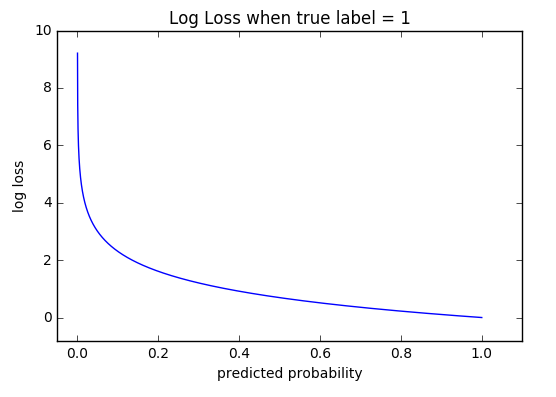
\includegraphics[width=\linewidth]{loss_functions/cross_entropy.png}
	\caption{Log Loss Function}
	\label{fig:logloss}
\end{marginfigure}


The three canonical loss functions as described by Vapnik \citep{vapnik1998statistical} are:
\begin{itemize} \item The 0-1 Loss – the simplest loss function mainly used in binary classification \begin{equation} L(y,\hat{y}) \end{equation}, resulting in an error of 0 if and only if $y == \hat{y}$. Otherwise the function will produce the value of 1. This does not however differentiate between different classes and types of errors. Variations of this function may thus be formulated by extending the simple loss function and make the resulting loss dependent on another function.
\item The squared loss – the equation used for regression defined as \begin{equation} L_{sq}(y,\hat{y}) \end{equation}  where the resulting error value is given by \begin{equation} (y-\hat{y})^{2} \end{equation} This is often the loss function of choice used in estimators such as linear regression and in many areas of machine learning \citep {Davidson-Pilon:2015:BMH:2851115}. One disadvantage of using the squared loss function is that it is sensitive to outliers, since the loss increases quadratically as the estimate moves away from the true value \citep {Davidson-Pilon:2015:BMH:2851115}. A loss function which is less sensitive to outliers is the absolute-loss function, given by: \begin{equation} L(y,\hat{y})=|y-\hat{y}|\end{equation} In this case, only the absolute value is taken of the difference between the estimated and real value. However this equation is not smooth where $(y-\hat{y})$ and thus may prove to be difficult to differentiate. 
\item Finally the probability estimation via the log loss is given by: \begin{equation} L_{log}(\hat{p})=-ln(\hat{p}) \end{equation} In this case rather than simply classifying the outputs into the different classes, we may also require the confidence level that a certain input belongs to a particular class. A variation of the log loss is the cross entropy which provides the possibility of classifying input into more than two classes. A depiction of the log loss function is given in Figure~\ref{fig:logloss}
\end{itemize}

In general loss functions must satisfy certain properties. Primarily they should not be expensive to compute \citep {Scholkopf:2001:LKS:559923} have only a small number of discontinuities in the first derivative and be convex in order to able to find a unique solution. In the case of regression problems another desirable property is resistance to outliers.

\begin{marginfigure}%
	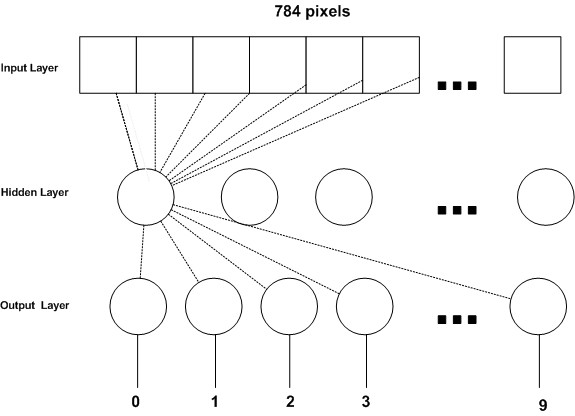
\includegraphics[width=\linewidth]{loss_functions/neural_network.jpg}
	\caption{Example Neural Network with Cross Entropy Loss Function}
	\label{fig:neural}
\end{marginfigure}

\subsection {Cost Functions}
Cost functions are generally based on loss functions which have been adapted to calculate the loss over a number of training examples. In this case it is assumed that there are $n$  samples or training examples for which an approximation for each of the errors $e$ in our model is to be calculated. Thus a cost function can be interpreted as representing a total error over all corresponding predictions for the training examples. Cost functions may also include  penalty terms, such as L1 or L2, for avoiding overfitting or underfitting. Some of the most widely used cost functions in regression are briefly explained here \citep {chai2014root}.
\subsection{MSE}
The Mean Squared Error for a dataset with $n$ training samples is given by summing the error $e$ for for all examples and calculating the squared difference from the true value $y$ and the prediction value $\hat{y}$.

\begin{equation}
MSE = {\frac{1}{n}\sum_{j=1}^{n}(y-\hat{y}})
\end{equation}

\subsection{RMSE}
RMSE has been widely used as a metric for model performance in meteorology, air quality and climate research study. The calculation is done by firstly obtaining the total square error which is the sum of the individual squared errors. Total square error is then divided by $n$. Large errors in this case have a greater influence on the total square error rather than smaller errors. While the rationale for squaring the individual error is to eliminate the sign \citep {willmott2005advantages}.
The formula is given below :-

\begin{equation}
RMSE = \sqrt{\frac{1}{n}\sum_{j=1}^{n}(y-\hat{y}})
\end{equation}

\subsection{MAE}

Calculation of MAE is simple, involving the summation of the absolute errors to the obtain the total error, then dividing by the total $n$. The formula is given below :
\begin{equation}
MAE = {\frac{1}{n}\sum_{j=1}^{n}\mid{y}-\hat{y}}\mid{}
\end{equation}

\subsection{Cross Entropy Loss}

In terms of classification cost functions,  Cross Entropy is the most frequently used.
\begin{equation}
\label{10}
L(y, \hat{y}) = -y \log(\hat{y}) - (1-y) \log(1-\hat{y})
\end{equation}

A practical example of Cross Entropy function as applied to Deep Neural Networks is now described.  Deep Neural networks are commonly good performers when used as classifiers, especially since these can be easily manipulated by changing their architecture, interconnections and activation functions according to specific requirements. However for such implementations the loss function of choice is almost always log loss, which is applied through softmax at the output layer \citep {DBLP:journals/corr/JanochaC17}. Lets assume, as an example, a dataset containing a large number of hand written digits from 0 to 9 as images and it is required to build a model  to recognize the hand written digits and categorize each input into 10 different classifications. The structure of the neural network used for this example is explained in Figure~\ref{fig:neural}. Each image of hand written digits is 28 x 28 pixels large, thus the input layer contains 784 neurons, while at the output layer we would require 10 neurons, each representing a digit from 0 to 9. The cost function that will be used in this example is the Cross Entropy function, as described in \ref{10}.

However, this formula is only suitable for one training example. Generally the weights for a deep neural network are updated after calculating the loss of a batched number of training examples. In this case the cost would need to be averaged over all training examples, and thus the function would be rearranged as follows:

\begin{equation}
L(Y, \hat{Y}) = -\frac{1}{m} \sum_{i=1}^m \left( y^{(i)} \log(\hat{y}^{(i)}) + (1-y^{(i)}) \log(1-\hat{y}^{(i)}) \right)
\end{equation}


In neural networks, it is required to compute how much the weights $w$ for each layer $j$  affect  the loss $L$. This can derived by finding the partial derivate of the cost function with respect to the weights, as follows:

\begin{equation}
\partial L / \partial w_j
\end{equation}

However it is generally not possible to find the partial derivative as described above directly. Instead by applying the chain rule it can be found how much the weights affect the activation functions for each layer and in turn how much these activation functions ultimately affect the loss. This can be formally described as follows:

\begin{equation}
\frac{\partial L}{\partial w_j} = \frac{\partial L}{\partial \hat{y}} \frac{\partial \hat{y}}{\partial z} \frac{\partial z}{\partial w_j}
\end{equation}

After finding the partial derivative of each function as described, the partial derivative of the cost function with respect to the weights can be substituted and finalised:

\begin{equation}
    \frac{\partial L}{\partial w_j} = \frac{\partial L}{\partial \hat{y}} \frac{\partial \hat{y}}{\partial z} \frac{\partial z}{\partial w_j}\newline
    = \frac{\hat{y} - y}{\hat{y}(1 - \hat{y})} \hat{y} (1-\hat{y}) w_j\newline
    = (\hat{y} - y) w_j.\newline
 \end{equation}


\input{terms/neuralnetwork_bp.tex}
\input{terms/noiseindatasets_is.tex}
\chapter{Online Learning Algorithms}
\label{ch:online-learning}\index{Online Learning|(}

\section{Introduction}

\begin{figure}
  \includegraphics{online_learning/traditional.pdf}
  \caption{The traditional batch train-test machine learning approach workflow.}
  \label{fig:traditional_ml}
\end{figure}

In the traditional machine learning approach depicted in Figure~\ref{fig:traditional_ml}, we usually have some historical data to train an algorithm on for predicting some future events \citep{oza_online_2005}. However, since most data environments are dynamic and will change, the trained model eventually becomes outdated. To tackle this, we usually automate model re-training based on a timeframe (i.e.\ weekly or daily basis). Although this helps with keeping the model up-to-date, this is still not enough. Even if we consider model re-training on a daily basis, the model would still be at least one day late. 

Furthermore, as \citet{pagels_what_2018} argued, no matter how good a specific model is, it would always be an imperfect representation of the problem. Moreover, to have the best prediction for today, we cannot rely on a model with knowledge about yesterday only. Enter online learning algorithms, a family of techniques that are modelled to consume as much data available (one sample at a time), as fast as possible, while continuously learning and adapting different learning parameters. In the following sections, we will dive deeper into the subject of online learning, and its particular usage.

\begin{figure}
  \includegraphics{online_learning/online.pdf}
  \caption{Basic workflow architecture of online learning.}
  \label{fig:online_ml}
\end{figure}

\section{Why use Online Learning?}

While being highly adaptable to dynamic underlying data structures since they make no statistical assumptions on the distribution of the data \citep{hoi_libol:_2014}, online learning techniques are also highly data efficient. Since online learning algorithms are only updated using the most recent data samples in the stream (as illustrated in figure~\ref{fig:online_ml}), such data samples are no longer stored or needed once the algorithm has passed over them, maintaining a much smaller data storage \citep{oza_online_2005}. Such algorithms are also very fast since only a single pass on a smaller data set is made, in contrast to the standard approach where the optimisation function needs multiple iterations over the entire dataset. Thus, as argued by \citet{hoi_online_2018}, online learning algorithms scale much better than the traditional approach.

As aforementioned, in offline machine learning, we load an entire dataset in memory, process it, then train a specific model, and then deploy the model into production. However, as more and more data is being generated, especially with the bright spotlight on Big Data, this methodology is proving to be more and more tedious. Some data sets are too large to fit into memory, even with distributed computing measures in place. Thus, online learning can drastically help in this scenario due to its small data storage property, especially when considered as online distributed computing and out-of-core computation \citep{zhang_projection-free_2017}, which is a huge plus.

To further extract the important usability of online learning, let us, as an analogy, consider the case of an online news portal where news articles are custom and shown to the users based on which categories that respective user usually tends to click. Pretending that a terrible disaster is happening or has happened on one specific day, and the government issues a 24-hour emergency evacuation; therefore, the majority of the user-base would start clicking on this news more and more. With the traditional batch approach, even with a re-training time of 24 hours, the system would fail to push this article to users who typically do not click on domestic affairs articles (i.e.\ users only interested in sports or entertainment). As a result, the same data content structure will be assumed by the algorithm even though there was a drastic change of events. 

In addition to this, given the same batch algorithm, after re-training in the following day, it would now start to suggest this article to a high percentage of the user-base, which by this time, such news might no longer be relevant or applicable.

Another small application resides in the online advertising domain. With different events and occasions happening every day, especially unscheduled or unforeseeable events which go viral, ads must stay relevant all the time to ensure the highest click-rate probability, and thus, must always synchronise to the affairs of the physical world. Ads must be intelligent enough to be aware of the hidden data distribution to adapt to data morphism.

In both examples, a traditional static model will fail due to being too slow to react to the dynamic underlying relationships present in the data. This problem is more formally known as concept drift \citep{schlimmer_incremental_1986}. The following section will further explain the notion of Concept Drift.

\section{Concept Drift} \index{Online Learning!concept drift}

Concept Drift occurs when the hidden context of the data changes. For instance, weather predictions are highly dependant on the season (the context), and as the seasons change so does the weather \citep{widmer_learning_1996}. As highlighted by \citet{krawczyk_online_2018, Gama2014ASO}, based on the distribution drift speed and severity, concept drift can be of four types as depicted in Figure~\ref{fig:cd}:

\begin{figure}
  \includegraphics{online_learning/cd.pdf}
  \caption{The four types of Concept Drift.}
  \label{fig:cd}
\end{figure}

\begin{enumerate}
\item \textbf{Sudden:}\index{Online Learning!sudden drift}
\textit{The data distribution is immediately changed to a different class.}
\item \textbf{Gradual:}\index{Online Learning!gradual drift}
\textit{The data distribution gradually transitions by having varying proportions of the different classes mixing together over time, until it completely changes to the new class.}
\item \textbf{Incremental:}\index{Online Learning!incremental drift}
\textit{The data distribution slowly morphs from one class to another.}
\item \textbf{Recurring:}\index{Online Learning!recurring drift}
\textit{The data distribution periodically transitions between previous classes.}
\end{enumerate}

\subsection{Dealing with Concept Drift}

Thus, to combat this, as the concept drifts, so must the model's transition function that maps the inputs to the outputs. Due to the constant model updates performed through online learning (sample by sample), the transition function would be dynamic and adapts to the changing distribution \citep{Gama2014ASO, hoi_online_2018, Lane:1998:AOL:3000292.3000339}. In addition to this, another approach is to have a sliding window that shifts with the data stream. The purpose of this window, as discussed by \citet{wozniak_hybrid_2011}, is to keep a set of instances that offer the best representation of the present data distribution. As newer data samples arrive in the stream, the window slides towards more recent instances, resulting in the exclusion of the oldest samples from the window. Online learning achieves this window technique through the 'forgetting rate' which sets how fast older data is discarded to make room for newer instances. 

\subsection{Forgetting Rate}\index{Online Learning!forgetting rate}

Even though the design for most online learning algorithms is for fast execution speeds and thus adapted from less complex algorithms, implementation challenges are also present. As argued by \citet{gepperth_incremental_2016}, this leads us to one of the most significant problems in online learning, Catastrophic Interference. The latter happens when the model abruptly forgets knowledge learnt for previous data. Most online learning algorithms have a forgetting rate parameter. This parameter allows the user to decide the speed at which the learning algorithm forgets old data; thus, how much data to retain. Moreover, the correct calibration of this rate is essential and challenging to perfect since a high value would result in catastrophic interference, while a lower value would result in the algorithm not adapting to the incoming samples in the stream. In addition to this, good initialisations are critical in this approach to steer away from slow convergence.

\section{Conclusion}

In this chapter, we introduced and discussed the sub-field of online learning algorithms concerning machine learning. Online learning is a highly useful tool that allows us to take machine learning to a whole other level by solving problems that otherwise would seem to be out of our technical ability. With the exponential importance for Big Data analytics, online learning arms us with the capabilities to process high-velocity data while also being fast to adapt to frequent changes in the data due to the ever-increasing data velocity.

\index{Online Learning|)}
\input{terms/regularisationofmodels_ja.tex}
\input{terms/sampleselectionbias_ac.tex}
\input{terms/semisupervised_mm.tex} 
\input{terms/structuralriskminimization_maf.tex}
\chapter{Synthetic Features}
\label{ch:synthetic features}\index{Synthetic Features|(}

\section{The problem}
Training a machine learning algorithm requires inputting some form of training data. This training data comprises of all the features from which the algorithm learns from and builds a model. This input is often referred to as the training dataset.

Whilst in concept the above seems straightforward, it often transpires that the various data-points provided in the training dataset do not fit a structure that is easily understood by the algorithm. For this reason, an important pre-processing step is needed to:

\begin{enumerate}
    \item Understand the original data well
    \item Subsequently, if and where needed, generate synthetic features
\end{enumerate}

If we look at the following example \citep{AlbertoTubeSpam}: It contains a number of records used to train a spam / ham classifier for comments on a YouTube video.

\begin{table}[ht]
    \centering
    \fontfamily{ppl}\selectfont
    \resizebox{\textwidth}{!}{\begin{tabular}{llllll}
      \toprule
      \textit{Video} & \textit{Comment ID} & \textit{Author} & \textit{Date} & \textit{Content} & \textit{Class} \\
      \midrule
      \textit{Psy} & \textit{LZQPQhLyRh9MSZYnf8djyk0gEF9BHDPYrrK-qCczIY8} & \textit{Evgeny Murashkin} & \textit{2013-11-08T17:34:21} & \textit{just for test I have to say murdev.com} & \textit{Spam}  \\
      \textit{Psy} & \textit{z13bgdvyluihfv11i22rgxwhuvabzz1os04} & \textit{Zielimeek21} & \textit{2013-11-28T21:49:00} & \textit{I'm only checking the views} & \textit{Ham}  \\
      \textit{Psy} & \textit{z13kxpqqssa0hlryd04cc1dxeyyngljjngk} & \textit{Tasha Lucius} & \textit{2014-01-19T13:25:56} & \textit{2 billion....Coming soon} & \textit{Ham}  \\
      \textit{Psy} & \textit{z12lg1vizrmsgxm3q23oij4aqrjxjdd1p} & \textit{Holly} & \textit{2014-11-06T13:41:30} & \textit{Follow me on Twitter @mscalifornia95} & \textit{Spam}  \\
      \bottomrule
    \end{tabular}}
    \caption{Sample of four rows from the Psy dataset from the YouTube comment training dataset.}
    \label{tab:sf_origdatasample}
\end{table}
\vspace{2mm}

Table \ref{tab:sf_origdataexplained} describes each feature in the original unmodified dataset.

\begin{table}[ht]
    \centering
    \fontfamily{ppl}\selectfont
    \resizebox{\textwidth}{!}{\begin{tabular}{ll}
      \toprule
      \textit{Feature} & \textit{Description} \\
      \midrule
      \textit{\makecell[tl]{Video}} & \textit{\makecell[tl]{The video this comment was written for. The relevance depends whether the \\ classification model is being built generically for all videos, or a per-video \\ specific model is also considered.}} \\
      \textit{\makecell[tl]{Comment ID}} & \textit{\makecell[tl]{Random comment ID generated by the YouTube comment board system. \\ This probably has no impact on the final class.}} \\
      \textit{\makecell[tl]{Author}} & \textit{\makecell[tl]{The author / account that generated the comment. This has relevance only if \\ this account has a lot of spam comments. \\ If that is the case, two things should happen, none of which are directly \\ related to the machine learning algorithm: \\ \quad - Maintain a blacklist of accounts that are probable spam (if a particular \\ \quad \enspace author often has flagged comments). \\ \quad - Block such accounts.}} \\
      \textit{\makecell[tl]{Date}} & \textit{\makecell[tl]{The date does not directly have a huge relevance on the classification of a \\ comment.}} \\
      \textit{\makecell[tl]{Content}} & \textit{\makecell[tl]{The comment body definitely has a big relevance in the classification result, \\ however, can the whole sentence be easily understood by the algorithm as \\ it is?}} \\
      \bottomrule
    \end{tabular}}
    \caption{Description of each feature in the original unmodified YouTube comment dataset.}
    \label{tab:sf_origdataexplained}
\end{table}
\vspace{2mm}

As one can see, there is very little input the machine learning algorithm can reliably take just from using the four features described above. One could easily realise this by asking oneself the following question (in plain English):

\emph{How can I describe the components of a comment well enough to decide whether it is probably spam or ham?}

One can therefore summarise this problem paradoxically as: \emph{Having enough data to solve the problem, but very little meta-data to actually understand it and solve it.}

\section{Ways of solving the problem}
A way of solving this problem is to apply a synthetic features approach, sometimes referred to as feature engineering. This is the generation of features derived from other existing features, in a way that can be more easily captured or understood by a machine learning algorithm \citep{LiFeatureEng}. It is a way of generating meta-data for the existing features in the original dataset.

In essence, the idea is to look at every available feature and for each determine the following:

\begin{itemize}
    \item Does the feature contain more than one feature within it? If so, try exploding it into sub-features and test.
    \item Does the feature contain too little information for any relevance, but could benefit from adding some context to it? If so, attempt at looking at other features that might be related, and produce new features as a result, and test.
    \item For each of the above, the original feature(s) might not be relevant anymore and be entirely replaced by the newly generated synthetic features instead.
\end{itemize}

What or how an explosion of features or a composite of features is generated depends on the very specific nature of the components involved and there is no generic formula behind it that works without some additional specificness. For example, two pairs of geo-coordinates probably qualify in giving a distance feature, however the formula applied here is specific to the geo-coordinates domain.

There is not a one-size-fits-all approach but rather it is more of an iterative approach with new synthetic features being outputted per iteration, following which one then assesses whether it is enough to generate a reliable machine learning model from the new features or not.

Following below is a practical example of this technique, using the dataset described at the introduction of this chapter.

\subsection{Analysing each feature} \index{synthetic-features!solving-problem-analysing-each-feature}

\begin{itemize}
    \item Video
    \begin{itemize}
        \item The video name / ID could be useful if a per-video classifier is also generated over and above the generic one. This together with other features could have some relevance.
    \end{itemize}
    \item Comment ID
    \begin{itemize}
        \item This feature does not have any relevance to the outcome whatsoever. It is a unique ID, built randomly, assigned to each comment. For this reason, it is out of scope for this discussion.
    \end{itemize}
    \item Author and Date
    \begin{itemize}
        \item As described earlier these two features independently do not have much of a direct impact on the outcome, however a synthetic feature could be generated which might have some form of effect on the outcome: A ratio of comment count over a time period for a particular author.
        The idea is to make it easier for the algorithm to detect a potential pattern related to volume over a typical short period, thus the definition of time period can be assigned via testing.
    \end{itemize}
    \item Comment
    \begin{itemize}
    \item The comment body is not an easy feature and it could grow into a number of features, however it is the most relevant input for this spam classifier.
    Quite a number of features could be exported from this comment, and most of them relate to natural language processing techniques \citep{CormackSMSFilter}. For this reason, output quality could also vary based on the language in context.
    Some example features that could be extrapolated:
    \end{itemize}
\end{itemize}

\begin{table}[ht]
    \centering
    \fontfamily{ppl}\selectfont
    \resizebox{\textwidth}{!}{\begin{tabular}{ll}
      \toprule
      \textit{Synthetic Feature} & \textit{Scope / Description} \\
      \midrule
      \textit{\makecell[tl]{Language}} & \textit{\makecell[tl]{This depends on the availabilities of various NLP implementations for \\ different languages, however one could have an indication of spam / \\ non-spam probabilities based on the comment languages for each \\ particular video.}} \\
      \textit{\makecell[tl]{Readability \\ score}} & \textit{\makecell[tl]{A readability score could be calculated per comment which gives an \\ indication on the quality of such text. An example of such a score \\ could be the \emph{Flesch Reading Ease} score.}} \\
      \textit{\makecell[tl]{Length \\ (excl. stop words)}} & \textit{\makecell[tl]{Very short or very long comments might have a probabilistic impact \\ on the outcome.}} \\
      \textit{\makecell[tl]{Presence of account \\ tags / URLs / emojis}} & \textit{\makecell[tl]{The presence of account tags (ex. a Twitter username), URLs or emojis \\ could increase probability of the comment being spam.}} \\
      \bottomrule
    \end{tabular}}
    \caption{Example of possible features that can be extracted from textual comments.}
    \label{tab:sf_commentextractedfeatures}
\end{table}
\vspace{2mm}

\subsection{Updated feature / data set} \index{synthetic-features!updated-feature-dataset}

Following the synthetic feature generation described above, the updated data set used as an example here would look as follows:

\begin{table}[ht]
    \centering
    \fontfamily{ppl}\selectfont
    \resizebox{\textwidth}{!}{\begin{tabular}{lllllllll}
      \toprule
      \textit{\makecell{Video}} & \textit{\makecell{Author Comments \\ in last minute}} & \textit{\makecell{Language}} & \textit{\makecell{Readability}} & \textit{\makecell{Length excl. \\ stop words}} & \textit{\makecell{Presence of \\ account tags}} & \textit{\makecell{Presence of \\ URLs}} & \textit{\makecell{Presence of \\ emojis}} & \textit{\makecell{Class}} \\
      \midrule
      \textit{Psy} & \textit{1} & \textit{EN} & \textit{94.3} & \textit{3} & \textit{No} & \textit{Yes} & \textit{No} & \textit{Spam}  \\
      \textit{Psy} & \textit{1} & \textit{EN} & \textit{103} & \textit{3} & \textit{No} & \textit{No} & \textit{No} & \textit{Ham}  \\
      \textit{Psy} & \textit{1} & \textit{EN} & \textit{83.3} & \textit{3} & \textit{No} & \textit{No} & \textit{No} & \textit{Ham}  \\
      \textit{Psy} & \textit{1} & \textit{EN} & \textit{32.6} & \textit{3} & \textit{Yes} & \textit{No} & \textit{No} & \textit{Spam}  \\
      \bottomrule
    \end{tabular}}
    \caption{Updated sample of the four rows from the Psy dataset from the YouTube comment training dataset now containing the synthetic features.}
    \label{tab:sf_updatedds}
\end{table}
\vspace{2mm}

Looking at the output in table \ref{tab:sf_updatedds}, the effect of synthetic features can immediately be appreciated, as with such new features more meaning is given to the original dataset.

Naturally the above contains just a sample, and one must experiment with:

\begin{itemize}
    \item more or less synthetic features
    \item a further iteration of synthetic features from the generated features
    \item a much bigger data-set (the example above is too small to build a reliable classifier)
    \item perform feature selection (such as Principal Component Analysis) to identify the features that actually matter and remove extra noise
\end{itemize}

Therefore, employing a synthetic feature approach on your dataset as a pre-processing step, should in general give you positive results.

\index{Synthetic Features|)}
\chapter[Tensor Processing Unit]{Tensor Processing Unit}
\label{ch:tensor-processing-unit}\index{Tensor Processing Unit|(}
A Tensor Processing Unit or TPU, is a proprietary Application-Specific Integrated Circuit\index{Application-SpecificIntegrated Circuit } (ASIC) used as an Artificial Intelligence accelerator \citep{jouppi2017datacenter}. It is designed and built by Google for use in their datacentre to power their products, including; Google Search, Google Translate, Google Photos and Gmail. Through Google's proprietary Accelerated Linear Algebra (XLA) compiler, binaries to run on TPUs are compiled from an XLA graph format produced by the TensorFlow libraries \citep{google}. 

Note that for the scope of this documentation, the architecture of the first generation TPUs is going to be explained, since it's the most well documented one. Further updates in the architecture are fairly similar to what will be discussed here and follow the same concepts, with the main difference being that newer generations are also used for training, instead of just inference. Therefore they support a truncated variant of the IEEE 754 single-precision floating-point format called bfloat16 instead signed 8-bit integers together with various other training optimizations.

\section{Background}\label{sec:background}

The motivation for Google to design and build a custom architecture on an ASIC, is due the shortcomings that come with Central Processing Units (CPUs) and Graphics Processing Units (GPUs) when used to run Artificial Neural Network\index{Artificial Neural Network} models. This is because 95\% of Google's applications in their datacentre run Neural Networks for inference, specifically; Convolutional Neural Networks (CNNs)\index{Convolutional Neural Network}, Multi-layer Perceptron Neural Networks (MLPs)\index{Multi-layer Perceptron} and Long short-term memory Neural Networks (LSTMs)\index{lstm} \citep{jouppi2017datacenter}. 

CPUs are sequential by nature, where each instruction is executed one at a time, which is really undesirable, and would require high clock speeds to get very high performance but with the expense of higher power consumption. In contrast GPUs are concurrent by nature, meaning that they can do several concurrent operations at once, therefore eliminating the need to have very high clock speeds, but it is only well suited for vector processing, hence their main use is Graphics Processing. In Machine Learning and specifically in Neural Networks, matrix operations are preferred as they speed up the computation by quite a big margin\citep{sato}.

Additionally, modern CPU and GPU architectures have performance issues due to their complex and sometimes non-deterministic ways of executing programs. This includes complex optimizations, like branch-prediction, out-of-order execution and multiprocessing \citep{paun2013determinism}. These algorithms are more tailored for throughput efficiency rather than having fixed latency \citep{jouppi2017datacenter}. Additionally, complex algorithms implemented in modern CPUs and GPUs, together with their high clock speeds, contribute to both a large area and higher power consumption. Google therefore designed their own custom AI accelerator chip around the necessary building blocks to run their Neural Network applications on, with the maximum possible efficiency.  

In order to understand why Google TPUs are designed as they are, an insight into the mathematics of involved in Neural Networks\index{Neural Network} is needed. The only computations done in Neural Networks involve only multiplications and additions, when excluding the activation function. While CNNs\index{Convolutional Neural Network} use convolution instead of multiplication, this report will explain the multiplication operations. This is because the input of a neuron is the sum of weighted (synapse weight) outputs of all the neurons in the previous layer, as represented in Equation~\ref{neuronsumofproducts}.

\begin{equation}\label{neuronsumofproducts}
Z = \sum_{i=1}^{n}x_{i}w_{i}
\end{equation}

Where $i$ is the number of neurons in the previous layer connected to the current neuron, $x$ is the output of each individual neuron in the previous layer, $w$ is the synapse weight present in the connection between the previous neurons to the current one. 

\section{Architecture}\label{sec:architecture}

Therefore as described in the previous section, a Multiply-Accumulate\index{Multiply-Accumulate} (MAC) block is the only computational block that is needed to perform the needed operations. Figure~\ref{fig:mac} illustrates a typical MAC block, where binary values A and B of length $[n:0]$ are multiplied, therefore producing a binary value C of length $[2n+1:0]$. C is then added to the accumulated binary value Y, and the Accumulator register is updated with the new accumulated binary value. The Accumulator Register's value is present on binary value Y.

\begin{marginfigure}
  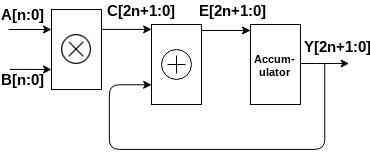
\includegraphics{graphics/tensor_processing_unit/tensor_processing_unit_mac.jpg}
  \caption{
    Multiply Accumulate Logic Block (Adapted from \citep{paquin}).
  }
  \label{fig:mac}
\end{marginfigure}

The MAC block alone does not contribute to good performance when a large data-set and complex Neural Networks are present, therefore TPUs implement it in a so called Matrix Multiplication Unit\index{Matrix Multiplication Unit} (MXU), which is basically a 2-dimensional array of MACs that operate in systolic form \citep{paquin}. The best intuitive way to understand how an MXU works is to visualize matrix multiplication as done in a layer of a Neural Network prior to activation\index{Activation Function}.

Consider the simple example shown in Figure~\ref{fig:neuralnetworkexample}, which shows a Neural Network\index{Neural Network} layer with 3 inputs and 2 neurons. Prior to applying the activation\index{Activation Function} function $f(x)$, the computation done is the same as described in Equation~\ref{neuronsumofproducts}, for each neuron, y1 and y2. 

\begin{marginfigure}
  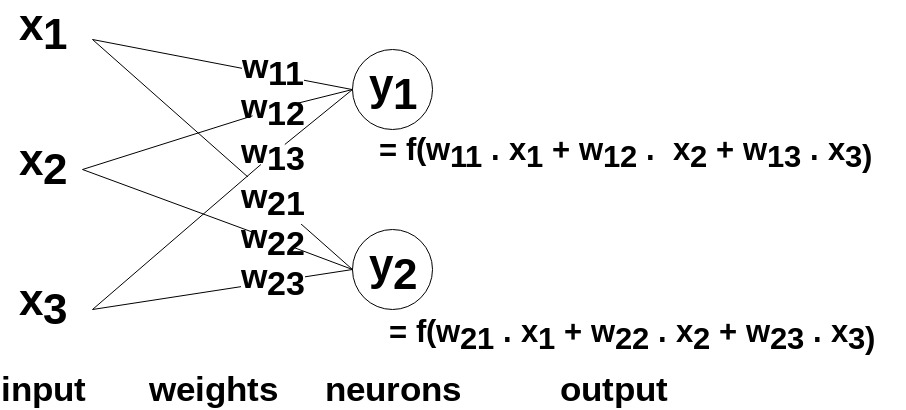
\includegraphics{graphics/tensor_processing_unit/tensor_processing_unit_nn.jpg}
  \caption{
    Example of a neural network layer with 2 neurons and 3 inputs (Reproduced from \citep{sato}).
  }
  \label{fig:neuralnetworkexample}
\end{marginfigure}

For this example an MXU needs to contain at least 6 MACs arranged in array of 2$\times$3, where 2 denotes the number of neurons and 3 denoting the number of inputs. Figure~\ref{fig:mxu} shows how such computation is done inside the MXU\index{Matrix Multiplication Unit} with just 1 example/instance X being inputted for inference, and since we are computing just 1 layer, the weights $w$ only need to be loaded once. 

\begin{figure}
  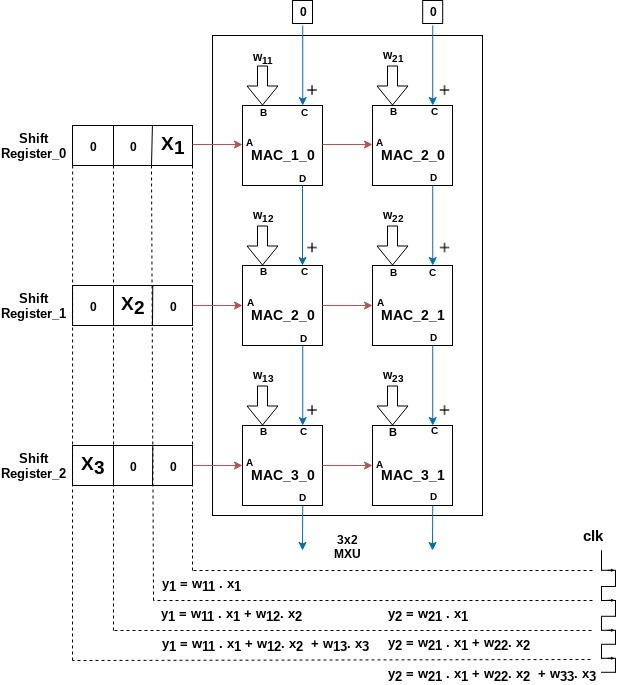
\includegraphics{graphics/tensor_processing_unit/tensor_processing_unit_mxu.jpg}
  \caption{
    Operation of a Simplified Matrix Multiplication block based on a 2 neuron layer example having 3 inputs (Adapted from \citep{sato}). 
  }
  \label{fig:mxu}
\end{figure}

Assuming input data X1, X2 and X3 are already loaded into their corresponding shift register and the weights $w$ are already present on one of their corresponding MAC inputs, the data flow with each clock cycle denoted by clk in Figure~\ref{fig:mxu}, which follows a systolic fashion. 

Prior to the computation, inputs A of all the MACs\index{Multiply-Accumulate} are reset to 0, while inputs B will have already been loaded with the weight values of the current layer. With each clock cycle the shift registers shift the data to the right into the MXU, where the A and B inputs are multiplied together and added with the value present at input C. In this manner the values of outputs D of the bottom most MACs will output the total sum of products on output D, with the bottom right most MAC being the last one to be updated after \textit{mn-m} clock cycles, where m is the number of inputs and n is the number of neurons. In this example the total amount of clock cycles needed is $2$ $\times$ $3$ $-$ $2$ $=$ $4$. In a Google's first generation TPU, there are 65,536 signed 8-bit MAC blocks in a 256$\times$256 array fashion that make up the MXU. The MXU in a TPU can compute both matrix multiplication and convolution \citep{sato}. After finally computing the sum of products, activation functions\index{Activation Function} are applied on each neuron's result.

Figure~\ref{fig:layouttpu} shows a high level representation of how all the components of the first generation TPU are connected internally, including the MXU\index{Matrix Multiplication Unit}. TPUs where designed to act as coprocessor with a host CPU, where they communicate together via a 3rd generation PCIe x16 bus. First generation TPUs were only designed for inference only, therefore the TPUs represent data only in a signed 8-bit integer, which has been proved that it is of sufficient precision for inference purposes \citep{jouppi2017datacenter}. 

\begin{figure}
  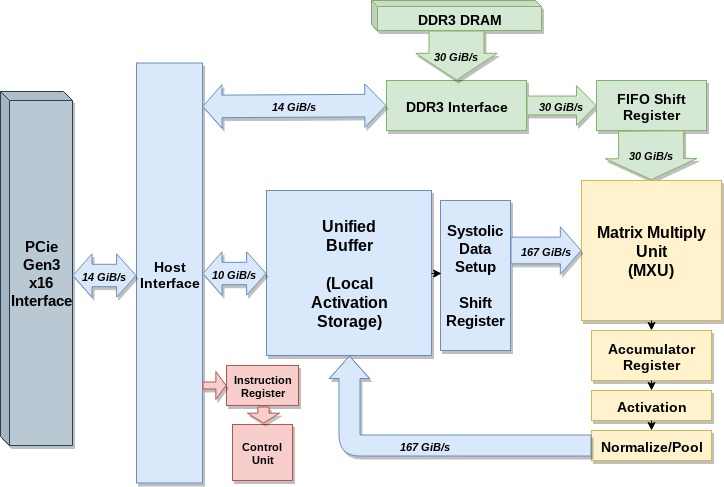
\includegraphics{graphics/tensor_processing_unit/tensor_processing_unit_arch.jpg}
  \caption{
    Internal Layout of a first generation TPU, showing the Control path (red), the Data paths for the weights (green) and for the activations/outputs (blue), together with the computational logic blocks (yellow) (Adapted from \citep{sato}).
  }
  \label{fig:layouttpu}
\end{figure}

As with any architecture, there is a Control path and a Data path. The Control path, which is denoted in red, serves the purpose of giving instructions to the TPU via the host CPU, like loading the data in registers, do multiplication and more. As for the Data path, two types of data are present. One being the weights, which are stored prior of inference and are denoted in green, while the other is the neurons activations/outputs, where its path is denoted in blue. As the weights are loaded only once before computing each layer, they do not require a high speed memory, so they are stored in a DDR3 DRAM, where later they are loaded into the MXU via a FIFO shift register. On the other hand, the neuron's activations/outputs, are stored by the host CPU in a high speed Unified Buffer through the PCI Express Interface. The Unified Buffer is where the activations of each neuron that are computed by the computational logic block are read and written, therefore it requires a high speed memory and interconnect bus. The Normalize/Pool block, processes the data to reduce its size or downsample it. As one can see the architecture is quite simple compared to other general purpose architectures like CPUs and GPUs. This allows Google to use a Complex Instruction Set Computer (CISC) instruction set with just a few instructions, since not many different operations are done \citep{sato}.

\index{Tensor Processing Unit|)}
\input{terms/transferlearning_jjd.tex}
\input{terms/roccurves_pb.tex}
\chapter{Standardization and Normalisation}

\label{ch:standardization-and-normalization}
\index{standardization and normalization|(}

Data \emph{standardization} and \emph{normalisation} are crucial data preprocessing stages in order to prepare the data for machine learning or data mining purposes\footnote{\url{http://www.dataminingblog.com/standardization-vs-normalization/}}.  Standardization is related to the act of centre-reducing the data and a common measure used is the \emph{standard deviation}\index{standardization and normalization!standard deviation}.  This is used in machine learning algorithms such as SVM \index{SVM} or regression \index{regression} problems.  On the other hand, normalisation is a process concerned with scaling or mapping the data in order to make it easier to work with \citep{patro2015normalization}.  Normalisation is useful in almost every machine learning algorithm (such as regression, kNN, neural networks) since it essentially cleans the data.  In this section we shall see a few standardization and normalisation techniques that are related to machine learning.



\section{Min-Max Normalisation}
Min-Max \index{standardization and normalization!Min-Max}is a linear normalisation technique and hence it does not alter the distribution of a data set.  Its goal is to transform the features of a data set to fit within a smaller and more specific range.  Normally this new range is set to $[0,1]$ (see Equation~\ref{eq:sn_min-max}) or $[-1,1]$.  This technique is sometimes called \emph{feature scaling}\index{standardization and normalization!feature scaling}.

\begin{equation}
% there is more than one form for this equation
\label{eq:sn_min-max}
x^{\prime}_{i} = \frac{x_{i} - x_{min}}{x_{max} - x_{min}}
\end{equation}

In equation~\ref{eq:sn_min-max} above, $x^{\prime}_i$ is the normalised value, $x_{i}$ is the unnormalised value and $x_{max}$ and $x_{min}$ are the maximum and minimum values found in dataset $X$ respectively.  

Equation~\ref{eq:sn_min-max-n} is a generic formula for this technique, where the range is specified at two arbitrary points $a$ and $b$:

\begin{equation}
\label{eq:sn_min-max-n}
x^{\prime}_{i} = (x_{max} - x_{min}) \times \frac{x_{i} - x_{min}}{x_{max} - x_{min}} + x_{min}
\end{equation}

 When compared to other normalisation techniques, the Min-Max is very effective whilst being a simple technique to implement \citep{al2006data}.  However, Min-Max is prone\emph{noise} and therefore produce unstable results as it is highly sensitive to \emph{outliers}\index{outliers} \citep{jain2005score}.

\section{Z-score/Zero-Mean Normalisation}
When applying \emph{z-score}\index{standardization and normalization!z-score} to a data set is the same as standardizing it.  Like Min-Max, this is a commonly used technique and it is easy to implement \citep{jain2005score}.  However, the Z-score or Zero-Mean normalisation affects the distribution of a data set such that it becomes \emph{normally distributed}\index{standardization and normalization!normally distributed}.  Figure \ref{fig:sn_normal-dist} \footnote{\url{https://www.kaggle.com/rtatman/data-cleaning-challenge-scale-and-normalize-data}} shows a plot of a normal distribution, also known as the \emph{Gaussian distribution}\index{standardization and normalization!Gaussian distribution}, compared with the original data (before transformation).

\begin{figure}
	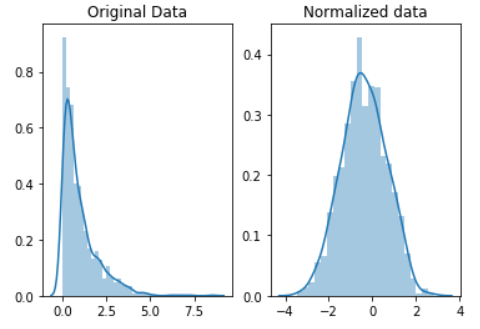
\includegraphics{standardization_and_normalisation/normal-dist.png}
	\caption{Normal Distribution example - notice the "bell curve" of the normalised data}
	\label{fig:sn_normal-dist}
\end{figure}

Equation~\ref{eq:sn_z-score} below shows how z-score is computed by normalising value $v_{i}$ of attribute $A$ to $v^{\prime}_{i}$:

\begin{equation}
\label{eq:sn_z-score}
v^{\prime}_{i} = \frac{v_{i} - \bar{A}}{\sigma_{A}}
\end{equation}

where $\bar{A}$ is the arithmetic mean and $\sigma_{A}$ is the standard deviation of attribute $A$.  When the minimum and maximum of attribute $A$ are unknown, this method is very useful and therefore preferred over Min-Max \citep{han2011data}.  This method is also highly applicable and effective for clustering algorithms such as \emph{K-means clustering}\index{standardization and normalization!K-means clustering} \citep{mohamad2013standardization} \citep{cheadle2003analysis}.

\section{Median Normalisation}
The Median normalisation technique works by calculating the \emph{median}\index{standardization and normalization!median} of a sample from a data set, then each element in the sample is divided by the median (see equation~\ref{eq:sn_median}).  This procedure repeated for every sample $s$ in a data set \citep{jayalakshmi2011statistical}.  

\begin{equation}
\label{eq:sn_median}
x^{\prime}_{i} = \frac{x_{i}}{median(s)}
\end{equation}

Equation~\ref{eq:sn_median-sub} is another way how Median normalisation is formulated, by subtracting the median from every element in sample $s$:

\begin{equation}
\label{eq:sn_median-sub}
x^{\prime}_{i} = x_{i} - median(s)
\end{equation}

For ~\ref{eq:sn_median} and  ~\ref{eq:sn_median-sub} $x_{i}$ is the unnormalised element in sample $s$.  Note that this technique known as an intra-slide normalisation because it works with whole arrays/samples of data.  Although this technique does not guarantee high accuracy, it is quite robust since it is much less sensitive to noise than Min-Max or Z-score \citep{jain2005score}.

\section{Sigmoid Normalisation}
The \emph{Sigmoid function}\index{standardization and normalization!Sigmoid function} can be used as a normalisation technique to scale values, usually between -1 and 1.  There are various forms of non-linear Sigmoid functions.  One example is the $tan$ Sigmoid function (refer to figure~\ref{fig:sn_tag-sig})which tends to speed up the normalisation process \citep{jayalakshmi2011statistical}.

\begin{figure}
	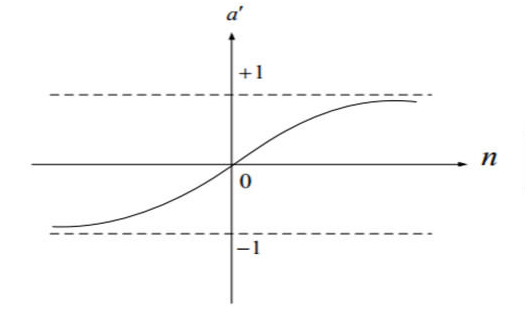
\includegraphics{standardization_and_normalisation/tan-sig.png}
	\caption{$Tan$ Sigmoid Function which can be used as a normalisation technique}
	\label{fig:sn_tag-sig}
\end{figure}

~\ref{eq:sn_tan-sig}is the equation of the $tan$ Sigmoid function:

\begin{equation}
\label{eq:sn_tan-sig}
x^{\prime}_{i} = \frac{e^{x} - e^{-x}}{e^{x} + e^{-x}}
\end{equation}

This normalisation technique is somewhat similar to the Min-Max method since it scales values to a specific range.  However, Sigmoid normalisation is more robust and shows greater efficiency \citep{jain2005score}.  Moreover, there is a more complex form of this technique which is the Double Sigmoid function \citep{cappelli2000combining}.

\section{Batch Normalisation}
\emph{Batch-norm}\index{standardization and normalization!Batch-norm} is a normalisation technique specifically developed for enhancing \emph{neural network}\index{standardization and normalization!neural network} training.  Before this technique was developed, neural networks were only normalised at the input layer only.  The problem with this was that if instability arises in one of the intermediate layers, then the layer would need to readapt to a new distribution thus slowing down the whole process.  This problem is known as \emph{internal covariate shift}\index{internal covariate shift} \citep{ioffe2015batch}.  Batch normalisation solved the problem by adding normalisation at each layer in the network.  Normalisation is done for every input neuron (one batch per neuron) found in the layer (see also figure~\ref{fig:sn_neural}).

\begin{figure}
	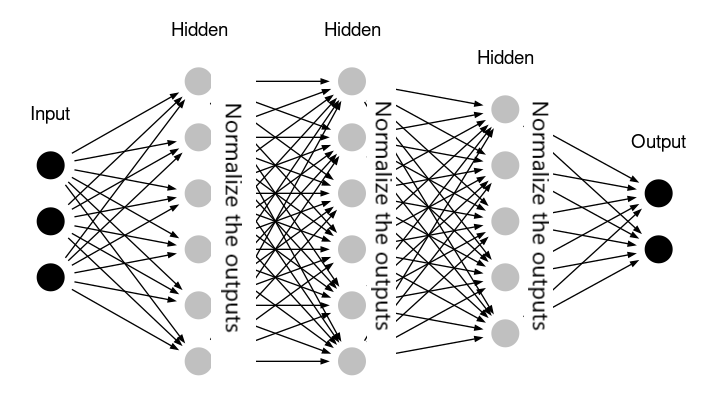
\includegraphics{standardization_and_normalisation/neural-network.png}
	\caption{Neural network with applied batch normalisation \url{https://mc.ai/batch-normalization-speed-up-neural-network-training/}}
	\label{fig:sn_neural}
\end{figure} 

\section{Conclusion}
From these few standardization and normalisation techniques, we have seen the importance to choose the right technique for the right data set (it is important to find out what kind of problem the data set is presenting - for example a regression problem, classification problem, a time-series, text mining and so on).  Some important features that a technique should have are: that it improves accuracy, reduces the training time, simplify the data and robustness to noise.

\index{standardization and normalization|)}
 %TODO

%%
% The back matter contains appendices, bibliographies, indices, glossaries, etc.

\backmatter



\bibliography{terms/featureselection_ab,terms/classification_cg,terms/empiricalriskminimisation_nf,terms/structuralriskminimization_maf,terms/bayesianmodels_kj,terms/neuralnetwork_bp,terms/roccurves_pb,terms/dimensionalityreduction_sc,terms/semisupervised_mm,terms/longshorttermmemory_nm,terms/regularisationofmodels_ja,terms/transferlearning_jjd,terms/sampleselectionbias_ac,terms/noiseindatasets_is,terms/onlinelearning_df,terms/crossvalidation_lmd,terms/confusionmatrix_df,terms/activationfunctions_km,terms/syntheticfeatures_fcm,terms/ensemblemethods_dv,terms/convolution_gebs,terms/evaluationmethods_ae,terms/generativemodels_pm,terms/hyperparameters_nm,terms/conceptdrift_mf,terms/standardizationandnormalisation_sm,terms/lossfunctions_ag,terms/tensorprocessingunit_pi} %TODO

\bibliographystyle{plainnat}

\printindex

\end{document}
